% =====================================================================
% ChartGenEval metric-suite paper (v6; floor-first framing)
% Venue-neutral two-column article for arXiv release.
%
% arXiv metadata: primary cs.SD; cross-list eess.AS;
% arXiv.org perpetual, non-exclusive license 1.0.
% All numbers are from the clean-split runs; the final records are archived
% under artifacts/records/ in the public ChartGenEval repository.
% =====================================================================
\pdfoutput=1
\documentclass[10pt,twocolumn]{article}
\usepackage[T1]{fontenc}
\usepackage[utf8]{inputenc}
\usepackage[a4paper,top=2.2cm,bottom=2.4cm,left=1.9cm,right=1.9cm,columnsep=0.8cm]{geometry}
\usepackage{newtxtext,newtxmath}
\usepackage{amsmath,cite,url}
\usepackage{graphicx}
\usepackage{booktabs}
\usepackage{placeins}
\usepackage{needspace}
\usepackage{balance}
\usepackage{titlesec}
\titlespacing*{\section}{0pt}{1.1em}{0.5em}
\titlespacing*{\subsection}{0pt}{0.9em}{0.4em}

% Discourage widows and orphans (e.g. the stray "a leaderboard." tail).
\widowpenalty=10000
\clubpenalty=10000
% Give the many full-width floats more room so figure-heavy pages pack
% tighter and leave fewer half-empty columns.
\renewcommand{\topfraction}{0.92}
\renewcommand{\bottomfraction}{0.85}
\renewcommand{\textfraction}{0.06}
\renewcommand{\floatpagefraction}{0.72}
\renewcommand{\dbltopfraction}{0.92}
\renewcommand{\dblfloatpagefraction}{0.72}
\setcounter{topnumber}{3}
\setcounter{dbltopnumber}{3}
\setcounter{totalnumber}{5}

\newcommand{\secref}[1]{Section~\ref{#1}}
\newcommand{\figref}[1]{Figure~\ref{#1}}
\newcommand{\tabref}[1]{Table~\ref{#1}}
\newcommand{\artifacturl}{\url{https://github.com/JacobLinCool/ChartGenEval}}

\title{\bfseries ChartGenEval: A Multi-Dimensional Metric Suite for
Rhythm-Game Chart Generation}

\author{Jhen-Ke Lin\\
  National Yang Ming Chiao Tung University\\
  \texttt{jacob.cs14@nycu.edu.tw}}
\date{}

% The first-page thesis graphic is part of the full-width title block so it
% cannot drift to a later page under two-column float placement.
\newcommand{\titlefigure}{%
  \begin{center}
    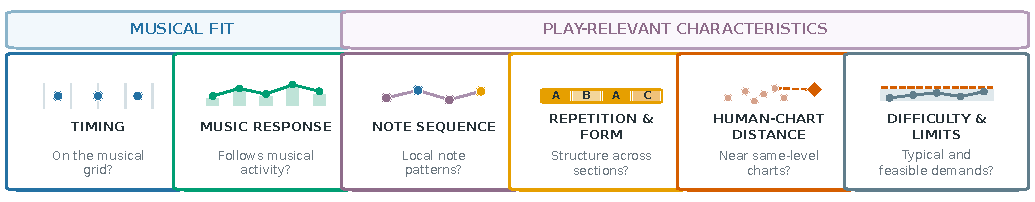
\includegraphics[width=0.96\textwidth]{figs/fig0_thesis.pdf}
    \refstepcounter{figure}\label{fig:overview}
    \parbox{0.94\textwidth}{\small
      \textbf{Figure~\thefigure: The six dimensions of ChartGenEval.}
      ChartGenEval organizes chart evaluation into six distinct questions,
      grouped by musical fit and play-relevant characteristics. Each
      dimension retains its own interpretation.}
  \end{center}
}

\makeatletter
\def\@maketitle{%
  \newpage
  \null
  \vskip 2em%
  \begin{center}%
    \let\footnote\thanks
    {\LARGE \@title \par}%
    \vskip 1.5em%
    {\large
      \lineskip .5em%
      \begin{tabular}[t]{c}%
        \@author
      \end{tabular}\par}%
    \vskip .7em%
    {\large \@date}%
  \end{center}%
  \par
  \vskip .6em%
  \titlefigure
  \vskip .8em%
}
\makeatother

\sloppy
\raggedbottom

\begin{document}
\maketitle

\begin{abstract}
A rhythm-game chart must fit its music and play well, yet one song
admits many valid note sequences. Agreement with one official chart
therefore conflates valid alternatives with errors. We introduce
ChartGenEval, a six-dimensional metric suite that uses the matched
official chart only for its authored timing map, never its note
placements. For injected whole-chart shifts of 15, 30, and 60\,ms, its
median grid-phase estimates match the true shifts. By contrast, every
primary chart-only output changes by less than 0.03 human standard
deviations.

ChartGenEval reports this timing profile alongside five higher-level
dimensions: note sequence, repetition and form, response to music,
same-difficulty human-chart distance, and difficulty and playability
limits. The dimensions remain separate, with no overall total. Nine
nonredundant corruption--measurement pairs met prespecified sensitivity
and invariance criteria on 80 held-out song groups; all 32 applicable
control checks passed. The stress tests also show why isolated proxies can be
misleading: common-pattern rewriting lowers language-model perplexity
by 37\%, while loop collapse raises self-similarity by 62\%. Together,
this automated six-dimensional profile can support fast comparison and
iteration of chart-generation models. Depending on their roles, its
outputs can serve as rewards, constraints, or monitoring signals in
training methods such as reinforcement learning.
\end{abstract}

\section{Introduction}\label{sec:intro}

Automatic chart generation for rhythm games maps audio to a playable
sequence of timed, typed notes. Research has progressed from
onset-detection methods to conditional sequence
models~\cite{donahue2017ddc,halina2021taikonation,takada2023genelive,
hanzen2025tcp}. Evaluation has not kept pace. A chart dictates what the
player must do and when; it answers to the music and to the player at
once. We organize evaluation around two requirements. \emph{Musical
fit} asks whether notes share the song's temporal structure and whether
chart activity follows the music's rise and fall. \emph{Play-relevant
characteristics} include learnable patterns, repetition with variation,
and demands appropriate to the requested difficulty. A chart is a
designed artifact: many note sequences can satisfy these requirements.

Existing methods answer useful but partial questions. The dominant
evaluation, placement F1 against the one official chart, quantifies
reconstruction: a valid alternative lowers overlap exactly as a flaw
does, and no comparison is possible when the song has no reference
chart. Optimizing agreement therefore rewards reproducing the official
answer and penalizes the departures that make charting a design problem.
Language-model (LM) likelihood quantifies model fit; distributional
and self-similarity statistics describe generated material; and player
or expert studies establish system-level experience. Each answers its
own question, and an aggregate of them hides its trade-offs.

Free note choice still leaves a timing question. Conventional
grid-based charts organize notes relative to a song's musical-time
framework. We measure this part of musical fit as alignment to an
external grid. The matched official chart supplies its authored
bar, meter, and tempo map, while its note placements are excluded as
targets. This split preserves freedom of note
choice while exposing chart-wide shifts that interval- and type-based
statistics cannot observe. The proposed grid-phase offset gives the
correct median estimate for injected shifts of 15, 30, and 60\,ms,
while every primary chart-only measurement remains nearly unchanged.

\textbf{ChartGenEval} automatically computes a profile across six
dimensions: timing, note sequence, repetition and form, response to
music, same-difficulty human-chart distance, and difficulty and
playability. Its outputs serve three roles: target signals for model
improvement, feasibility constraints, and monitoring signals for model
comparison and error analysis. These roles remain separate, so each
dimension keeps its meaning.

Controlled corruptions provide the sensitivity evidence. Starting from
a human chart, we apply a dose-controlled transformation designed to
impair one property and ask whether its target measurement responds while
the applicable control checks remain unchanged. The nine transformations cover dense
timing jitter, sparse timing errors, a whole-chart shift, note-type
shuffling, loop collapse, common-pattern rewriting, density scaling,
burst insertion, and bar shuffling. We selected and revised candidate
measurements on 40 development songs, then evaluated ten prespecified
corruption--measurement pairs on 80 held-out song groups. The results
meet all target and control criteria; one algebraically equivalent pair
leaves nine nonredundant tests (\secref{sec:sensitivity}). Development
stress tests further show that LM perplexity can favor common-pattern
rewriting, self-similarity can favor loop collapse, and chart-only
measurements miss a constant chart--audio shift.

Our contributions are:
\begin{enumerate}
\item \textbf{Automated six-dimensional feedback.} ChartGenEval
  computes separate signals for timing, note sequence, repetition and
  form, response to music, human-chart distance, and difficulty and
  playability. These signals can support model comparison, iteration, and
  reward-based training.
\item \textbf{Controlled-corruption evidence.} Nine dose-controlled
  corruptions yield nine nonredundant held-out tests of target response
  and specified invariance checks. The same design exposes proxy sign reversals
  and the global-shift blind spot of chart-only measurements.
\item \textbf{Chart-specific measurements.} The suite adds a grid-phase
  offset and five development-stage components for chart--audio response,
  long-form structure, and human-chart distance.
\end{enumerate}

\section{Related Work}\label{sec:related}

\textbf{Reference-chart agreement.} DDC and Gen\'eLive! report F-scores
for predicted placements, while TCP reports onset and onset-plus-type
F1 together with local pattern
recall~\cite{donahue2017ddc,takada2023genelive,hanzen2025tcp}. Their
tolerances and aggregation differ: DDC uses $\pm20$\,ms, Gen\'eLive!
uses $\pm50$\,ms, and TCP defines tolerances as fractions of a bar.
TaikoNation instead compares 23\,ms binary frames and pattern
spaces~\cite{halina2021taikonation}. These are reconstruction estimands and
inherit the single-reference limits described in \secref{sec:intro}.

\textbf{Unpaired and human-anchored evaluation.} DDC uses LM perplexity
and token accuracy to evaluate held-out model
fit~\cite{donahue2017ddc}. Symbolic-music and
text-generation work contributes diversity, feature-distribution,
self-similarity, and set-level repetition
statistics~\cite{li2016diversity,zhu2018texygen,yang2020evaluation,dong2020muspy,
wu2020jazz}. Human studies answer another question. MuTE validates a
reference-aligned piano-arrangement measure against expert
ratings~\cite{gover2022mute}; Gen\'eLive! reports professional deployment
feedback~\cite{takada2023genelive}; and Mania Archetype combines
reference similarities with ratings from eight experienced
players~\cite{wang2024mania}. ChartGenEval supplies the automatic measurements and
corruption-sensitivity evidence that such human studies can build on.

\textbf{Metric stress tests and timing.} SCHmUBERT constructs
non-musical piano rolls that match framewise self-similarity
statistics~\cite{plasser2023schmubert}. Fr\'echet Music Distance is tested with
pitch and velocity perturbations, but remains a set-level embedding
distance~\cite{retkowski2025fmd}. STRUM reports reference-onset F1 after
a per-song global-offset search~\cite{opria2026strum}; ChartGenEval
reports the whole-chart grid-phase offset as a chart-level measurement
without using reference notes as targets. Our 6\,ms timing tolerance follows temporal discrimination
research~\cite{friberg1995jnd,london2012hearing}
(\secref{sec:timingmethod}).

\section{Methods}\label{sec:methods}

\subsection{ChartGenEval metric suite}\label{sec:suite}

ChartGenEval automatically computes six groups of measurements.
Controlled corruptions test target sensitivity across doses, while
applicable control checks test invariance. Table~\ref{tab:suite} distinguishes the
measurements proposed here from adaptations of established chart
statistics and states the strongest evidence available for each role.

\begin{table*}[t]
\centering
\footnotesize
\setlength{\tabcolsep}{5pt}
\renewcommand{\arraystretch}{1.15}
\begin{tabular}{@{}p{0.135\textwidth}p{0.375\textwidth}p{0.165\textwidth}p{0.235\textwidth}@{}}
\toprule
Construct & Primary output and reading & Origin & Evidence basis \\
\midrule
Timing & Grid clean rate and residual tail; whole-chart grid-phase offset & Proposed chart-to-grid profile & C1, C1s, C2 held-out tests using the authored grid \\
Note sequence & LM loss as description; unseen-transition penalty as a one-sided familiarity check & Adapted $n$-gram statistics & C3 held-out test (transition familiarity) \\
Repetition and form & 4-gram typicality; ABAB reciprocity; stagnation--alienation proxy & Adapted 4-gram score; two proposed measures & C4, C5, C8 held-out tests (one 4-gram axis); new measures development only \\
Response to music & Bar-level density--energy rank correlation; run-head onset support & Two proposed measures & Development only \\
Human-chart distance & Mean distance to 20 nearest training charts in a 32-dimensional chart representation & Proposed chart-specific instantiation & Development only \\
Difficulty and limits & Density and strain typicality; overload and density-spike limits & Adapted statistics; proposed calibration & C6, C7 held-out tests (density typicality, spike limit) \\
\bottomrule
\end{tabular}
\caption{ChartGenEval constructs, origins, and evidence boundaries. Each
construct's required timing, audio, grid, or reference anchor is given
in Methods (\secref{sec:data}, \secref{sec:layers}). ``Proposed'' marks
measurements defined in this work; their basic statistics may already be
established. Held-out evidence refers only to the named outputs.}
\label{tab:suite}
\end{table*}

All ChartGenEval outputs are computed automatically, but they serve
different roles. Directional outputs can act as rewards or penalties,
playability checks as constraints, and descriptive outputs as monitoring
signals. A training method, including reinforcement learning, can choose
and weight these signals for its task.

The proposed measurements target gaps left by individual chart
statistics. The \emph{whole-chart grid-phase offset} searches shifts from
$-250$ to $+250$\,ms against a fixed lattice of bar, beat, and
eighth-note anchors. To test whether activity follows the music's rise
and fall, the \emph{density--energy response} is the Spearman
correlation between hits per second and linear mel energy in authored
bar windows. It is unavailable with fewer than eight windows or when
the song's 90th--10th percentile energy range is below 5\% of its
median. The \emph{run-head onset support} is the fraction of
rhythmic-group heads whose maximum spectral flux within three mel frames
($\approx\pm35$\,ms) reaches the song's 60th-percentile threshold. A
new group begins after an inter-onset interval of at least 0.25\,s,
preventing dense runs from dominating the denominator.

For long-form structure, \emph{reciprocity} divides the chart into
two-bar phrases on sixteenth-note slots. A tolerant,
chance-corrected rhythm similarity is multiplied by chance-corrected
color agreement. If $S(i,j)$ denotes this product with one-slot
tolerance, the score is the phrase mean of
$S(i,i+2)[1-S(i,i+1)]$: material returns after the intervening phrase
without rewarding adjacent copy-paste repetition.

The \emph{stagnation--alienation proxy} operates on active-bar rhythm
and color fingerprints. A bar is stagnant when it is the fourth or
later member of a consecutive similarity-$\geq.8$ run, or when every
eligible 16-note color window is exactly periodic with period at most
four. A bar is alienated when no bar with similarity at least .75
occurs within 32 bars in either direction. The raw output is the
fraction of active bars in the union of these sets. We interpret the
output as a structural signal. Finally, the \emph{human-chart
distance} represents each chart with 32 interval, note-type, density, and
variety features. Features are standardized within course; the raw distance
is the mean Euclidean distance to the 20 nearest training charts of
that course. Its bounded display score is $\exp(-g/a)$, where $g$ is
the raw distance and $a$ is the course's 90th percentile leave-one-out
distance.
The representation is chart-specific; its entropy, bigram, and
nearest-neighbor primitives are established statistics.

\subsection{Data and timing references}\label{sec:data}

We use taiko-style chart files and associated audio gathered from
community resources available online. The chart files transcribe the
official difficulty courses; we use them as human reference charts.
Because the underlying charts and audio are potentially copyrighted
content, the corpus itself is not distributed. Source rows are grouped
by underlying song, with inconsistent source mappings rejected. The
training and test splits serve different purposes. The training split
has 924 source rows covering 813 unique song groups and 3{,}880 course
charts. We use these charts to fit the calibration and LM. The test
split has 140 source rows forming 120 song groups. The first 40 groups
contain 170 human charts and form the development panel for metric and
corruption design, figures, and system profiles. The remaining 80
groups contain 333 course charts and form the held-out panel for
confirmatory tests. The dataset also has a validation split of 80 song
groups, which is not used in the reported analyses. Across the
development and held-out analyses, controlled corruptions cover all 120
test songs: 40 for development and 80 for held-out confirmation. The
public-system comparison uses the 40 development songs.

The five additional proposed components were selected and revised on
the development panel, so their evidence remains exploratory.
Appendix~\ref{app:protocol} documents panel construction and the full
analysis specification.

Timing requires an external song-timing reference. The primary grid
comes from the matched official chart file's authored per-bar
timestamps, meter, and tempo metadata. Its note times and note types
are never used as targets: the official file supplies the timing map,
not a single correct note sequence. This retains the map's precise
authored bar structure while allowing generated charts to make
different valid note choices within the same musical-time framework.
We never use the grid declared by the generated chart, because that
would let the generator define its own reference.

We also evaluate audio-estimated downbeats as a development-stage
alternative when an authored timing map is unavailable. On 39 of the 40 development
songs, the estimated beat period is within 2\% of the metadata-based
period; the remaining song differs by 2.39\%. Absolute-offset reporting
uses the authored grid, which fixes bar phase directly from the timing
map. Only courses with an authored timing map enter the held-out timing
analysis; timing measurements are unavailable for the remaining courses.

\subsection{Measurement roles and difficulty calibration}\label{sec:layers}

Each chart is a sequence of timed, typed notes. We organize the raw
measurements around the six question groups in \figref{fig:overview},
which divide between the two requirements of \secref{sec:intro}.
Musical fit is agreement between what is heard and what is played, so
timing and response to music require the song. The other four groups do
not require audio and describe play characteristics; the proposed
structure measurements additionally require a metrical grid. The adapted chart-side primitives are a
smoothed trigram LM, unseen-transition rate, note rate, local density,
short-interval load, entropy, and unique or repeated 4-grams. We retain
trigram negative log-likelihood (NLL) as a description of LM fit;
perplexity is its exponential. We transform NLL separately into a
course-conditioned band score, termed \emph{pattern-IC typicality}.
Unseen-transition rate supplies a one-sided \emph{transition-familiarity}
check: an unseen trigram is unfamiliar to the training corpus, not
semantically invalid. The proposed structure, audio-response, timing,
and human-gap measurements are defined in \secref{sec:suite}.

We turn each selected feature into a
\emph{same-difficulty band score}. For every course and selected
feature, let $l$ and $u$ be the 10th and 90th percentiles of the training
charts and let $h=\max((u-l)/2,10^{-9})$ be the protected half-width.
The distance is symmetric at the two edges:
\begin{equation}
\begin{aligned}
d(x)&=
\begin{cases}
(l-x)/h, & x<l,\\
0,       & l\leq x\leq u,\\
(x-u)/h, & x>u,
\end{cases}\\
s(x)&=\frac{1}{1+d(x)^2}.
\end{aligned}
\label{eq:band}
\end{equation}
Thus a chart scores 1 inside the band, and equal departures below and
above it receive equal scores. We also retain the signed distance so
that large departures do not collapse to the same near-zero score.

This score measures how unusual a chart is for the requested
difficulty; it does not by itself say whether the chart is good. Some
measurements have a declared undesirable direction, such as excess
load beyond a course-relative limit; these use separately named
one-sided scores. Transition familiarity is also one-sided relative to
the training corpus, without implying semantic invalidity. Family
measurements without a declared calibration remain raw descriptions.
Entropy, density, and repetition have no universal direction: each can
be too low or too high. The controlled corruptions show that targeted
changes often move these values away from the human band. An unusual
chart that remains playable and follows the music may still be creative
(\secref{sec:discussion}).

Playability limits remain separate, non-compensable feasibility checks. On human charts in the
development panel, 88\%, 89\%, and 97\% score at least 0.99 on the
note-rate, short-interval, and density-spike checks, respectively.
Values such as estimated global shift remain descriptive.

\subsection{Measuring timing against the song}\label{sec:timingmethod}

We treat grid deviations below 6\,ms as within tolerance, at the scale
of the published just-noticeable difference for short
intervals~\cite{friberg1995jnd}. Larger errors are reported in three
ranges: above 6, 12, and 18\,ms. We also compare consecutive note
intervals using a tolerance of
$\max(6\,\mathrm{ms},2.5\%\times\mathrm{IOI})$. Every note is counted
as within tolerance, above one of the three ranges, or unmatched.
Unmatched generated notes remain in the denominator, so added off-grid
notes lower the within-tolerance rate. The measure has no reference-note
recall term: deleting unmatched generated notes can raise the rate. We
therefore interpret it together with note count and same-difficulty
density. We summarize each chart first, then report medians and tails
across charts.

A common shift $\delta$ leaves every inter-note interval unchanged:
\begin{equation}
(t_{i+1}+\delta)-(t_i+\delta)=t_{i+1}-t_i.
\label{eq:shift-invariance}
\end{equation}
The note types are also unchanged. Chart-only measurements built from
these intervals and types therefore stay unchanged or nearly unchanged.

Nearest-grid matching can miss a constant shift (\figref{fig:timing}).
On a dense grid, each shifted note may simply be paired with another
nearby grid point. We therefore estimate one offset for the whole chart.
Let $G_k$ be the fixed bar, beat, and eighth-note grids, and let
$d(x,G_k)=\min_{g\in G_k}|x-g|$. For note times $t_i$, we score a
candidate shift by
\begin{equation}
\begin{aligned}
S(\delta)
 &= \sum_k w_k\,\frac{1}{n}\sum_i
 \left[1-\frac{d(t_i-\delta,G_k)}{\tau}\right]_+,\\
\hat{\delta}
 &= \operatorname*{arg\,max}_{\delta\in[-250,250]\,\mathrm{ms}}
 S(\delta),
\end{aligned}
\label{eq:phase-offset}
\end{equation}
where $[z]_+=\max(z,0)$, $\tau=12$\,ms, and the bar, beat, and
eighth-note weights are 0.2, 0.3, and 0.5. We search in 0.5\,ms steps.
The authored grid comes from the official chart's timing map, not its
note sequence; the audio-estimated grid comes from audio downbeats.
Combining the three grids resolves most periodic ties; the
smallest-magnitude offset is chosen for near-ties.
Both timing summaries require one of these external grids. If neither an
authored map nor an audio-estimated grid is available, timing is reported
as unavailable. BPM alone supplies a period but no phase, so it cannot
serve as a timing reference.

\begin{figure*}[t]
\centering
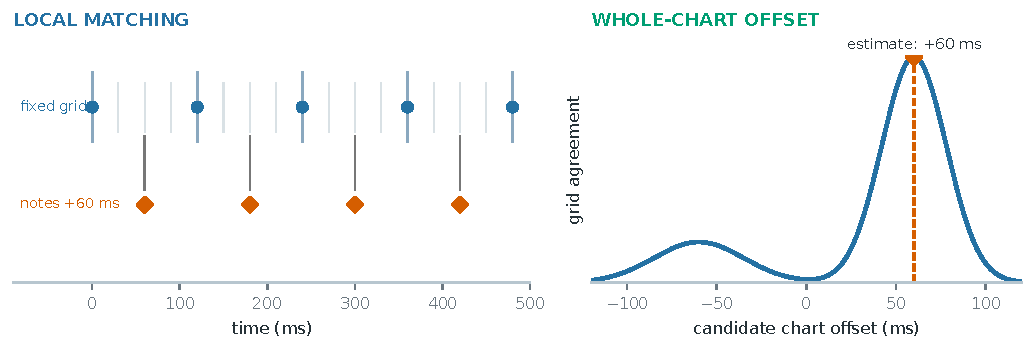
\includegraphics[width=0.94\textwidth]{figs/figT_timing_alignment.pdf}
\caption{Why timing needs a whole-chart estimate. \textbf{Left:}
nearest-grid matching can pair shifted notes with different subdivision
points and report small local errors. \textbf{Right:} a schematic agreement
curve over candidate whole-chart offsets; the curve peaks at the injected
$+60$\,ms shift. The grids are fixed before evaluating the generated chart.}
\label{fig:timing}
\end{figure*}

\subsection{Controlled corruptions and acceptance rules}
\label{sec:probes}

\begin{table*}[t]
\centering
\footnotesize
\setlength{\tabcolsep}{4pt}
\begin{tabular}{@{}p{0.30\textwidth}p{0.18\textwidth}p{0.46\textwidth}@{}}
\toprule
Controlled corruption (strength) & Changes & Prespecified response \\
\midrule
C1 timing jitter ($\pm$10/20/30\,ms) & note timing &
timing clean rate $\downarrow$ \\
C1s sparse timing errors (nominal 0.5/1/2\%, $\pm$60\,ms) & a few note times &
absolute timing-error p99 $\uparrow$ \\
C2 global shift (+15/30/60\,ms) & chart--audio alignment &
absolute grid-phase offset $\uparrow$ \\
C3 note-type shuffle ($p{=}0.2/0.4/0.8$) & local transitions &
transition familiarity $\downarrow$ \\
C4 loop collapse ($p{=}0.3/0.6/1$) & repetition and form &
4-gram typicality $\downarrow$ \\
C5 common-pattern rewrite ($p{=}0.3/0.6/1$) & pattern variety &
4-gram typicality $\downarrow$ (one effective axis) \\
C6 note-rate scale ($\times$0.5/1.5/2) & difficulty fit &
note-rate typicality $\downarrow$ \\
C7 burst insert (2/4/8 clusters) & local overload &
density-spike limit $\downarrow$ \\
C8 bar-order shuffle ($p{=}0.3/0.6/1$) & global form &
4-gram typicality $\downarrow$ \\
\bottomrule
\end{tabular}
\caption{Controlled corruptions and their nine nonredundant target
readings. C3--C5 preserve note times, while C4 and C6 preserve or
control density. C5 originally named two algebraically equivalent
4-gram outputs; we count them as one effective axis. Pattern-IC
typicality and raw trigram NLL remain direction-free secondary analyses.
Appendix~\ref{app:corruptions} provides visual before--after examples and
the complete transformation specifications.}
\label{tab:probes}
\end{table*}

The development response matrix is descriptive. It reports standardized
maximum-dose changes and the per-chart net direction: the fraction
moving up minus the fraction moving down relative to each chart's intact
version. Appendix~\ref{app:protocol} gives the complete development
calculation and the independent-LM check for C5.

We evaluated ten prespecified corruption--measurement rows on 80
held-out song groups. Five deterministic corruption replicates were
averaged within chart and dose, and courses were averaged within song,
leaving songs as the inferential unit. Each test used an oriented dose
correlation and a maximum-dose-minus-sham contrast. We computed
song-cluster bootstrap intervals and applied Bonferroni-adjusted 99.5\%
intervals across the ten rows. A response met the criterion when at
least 72 songs were evaluable, every required control passed,
and both adjusted upper bounds were below zero.
Appendix~\ref{app:protocol} provides the full protocol.

The controls match the invariance claimed by each measurement family.
They include exact re-evaluation, a joint shift of notes and grid, a
Don--Ka color bijection for timing and density, and a whole-chart
translation for chart-only measurements. A failed control prevents a
target response from being counted as supported.

\subsection{Evaluated systems}\label{sec:systems}

We evaluate five public generators spanning three note formats: Taiko
note types, timing-only onset streams, and osu! position-based objects.
Two systems produce Taiko note types: Mapperatorinator
v32~\cite{mapperatorinator}, a community-developed, MIT-licensed
framework for multi-gamemode osu! beatmap generation evaluated here in
taiko mode, and the FDG-published TaikoNation
system~\cite{halina2021taikonation}, run from the authors' public
research repository.
Three systems enter only the timing
and music-response measurements: Dance Dance Convolution's onset
pipeline (ddconset)~\cite{donahue2017ddc}, the public timing-only
configuration of Gen\'eLive!~\cite{takada2023genelive}, and
AutoOsu~\cite{autoosu}, an osu! difficulty-targeted generator. All
systems chart the same 40 development songs from audio in
their public inference configurations. We did not train or fine-tune
these systems on this corpus, although overlap between these commercial songs and the
systems' own training data cannot be excluded
(\secref{sec:limitations}). Course mappings are as follows.
Mapperatorinator uses the corresponding Taiko course.
Gen\'eLive's Beginner, Easy, Medium, Hard, and Challenge settings map to
Easy, Normal, Hard, Oni, and Ura; when a song has no Ura chart,
Challenge uses Oni as its reference course. Single-setting systems
use the declared Oni reference. Format conversion into the evaluation
event stream is shared within each note format
(\secref{sec:systemresults}). Human
charts of the same songs provide the reference row. Systems that
condition on difficulty produce one chart per available course (170 or
200 charts); the others produce one per song (40). We report these
profiles as descriptive development analyses.

\section{Results}\label{sec:results}

\subsection{Nine effective tests meet the held-out criteria}
\label{sec:sensitivity}

All ten prespecified rows met both response criteria, all 32 applicable
control checks passed, and every analysis retained all 80 song clusters
(\tabref{tab:confirmation}). The two C5 rows are algebraically
equivalent, so the result represents nine nonredundant
corruption--measurement pairs across seven effective output axes.

\begin{table*}[t]
\centering
\scriptsize
\setlength{\tabcolsep}{3.5pt}
\begin{tabular}{@{}llrll@{}}
\toprule
Pair & Primary response & Courses & $\bar\rho_{\mathrm{dose}}$ [99.5\% CI] &
$\overline{\Delta}_{\mathrm{max-sham}}$ [99.5\% CI] \\
\midrule
C1  & timing clean rate & 333 & $-.744\;[-.815,-.667]$ & $-.502\;[-.558,-.446]$ \\
C1s & absolute timing-error p99 & 332 & $-.234\;[-.344,-.134]$ & $-.306\;[-.508,-.144]$\,ms \\
C2  & absolute grid-phase offset & 333 & $-.916\;[-.981,-.826]$ & $-55.58\;[-61.43,-49.83]$\,ms \\
C3  & transition familiarity & 333 & $-.800\;[-.856,-.737]$ & $-.231\;[-.262,-.199]$ \\
C4  & 4-gram typicality & 333 & $-.445\;[-.573,-.312]$ & $-.165\;[-.226,-.108]$ \\
C5  & 4-gram typicality & 333 & $-.358\;[-.459,-.258]$ & $-.131\;[-.189,-.078]$ \\
C6  & note-rate typicality & 333 & $-.693\;[-.784,-.579]$ & $-.582\;[-.672,-.483]$ \\
C7  & density-spike limit & 333 & $-.940\;[-.950,-.930]$ & $-.619\;[-.644,-.593]$ \\
C8  & 4-gram typicality & 330 & $-.589\;[-.728,-.435]$ & $-.224\;[-.293,-.156]$ \\
\bottomrule
\end{tabular}
\caption{Held-out results on 80 song groups. Larger
oriented values are better, so target sensitivity appears as a negative
dose correlation and a negative maximum-dose-minus-sham contrast. All
nine effective pairs meet the prespecified criteria; intervals are
family-wise 99.5\% song-cluster bootstrap intervals. C5 reports one of
two algebraically equivalent output rows.}
\label{tab:confirmation}
\end{table*}

All 32 controls were exactly invariant. C1s retained 332 complete
courses and C8 retained 330; the other pairs retained 333. Sample counts
and exclusion reasons appear in Appendix~\ref{app:protocol}.

\paragraph{C5 contributes one effective axis.}\label{sec:dependency}
Repeated 4-gram rate is exactly one minus unique 4-gram rate. Their
mirrored symmetric-band scores are therefore identical up to
floating-point roundoff. The two prespecified C5 output names do not
provide independent corroboration; C5 supports one effective 4-gram
repetition/uniqueness response.

\subsection{External time detects chart--audio shifts}
\label{sec:anchorresults}

A chart can have plausible density, patterns, and note types while being
late relative to the music. C2 shifts every note by 15, 30, or 60\,ms.
On the development panel, no primary chart-only output changes by more
than 0.03 human standard deviations because interval- and type-based
measurements are invariant to a common translation.

Nearest-grid matching also misses the shift: a dense lattice can pair
each shifted note with a different nearby subdivision. The grid-phase
offset search instead returns median estimates of 15.00, 30.00, and
60.00\,ms from both reference sources. For every source and shift, at
least 169 of 170 charts are within 3\,ms of the injected value. Run-head
onset support also responds at note onsets (net direction $-0.74$ to
$-0.88$ across strengths) while remaining unchanged when note times are
preserved. Under dense timing jitter, the fraction of notes within
6\,ms falls in every chart at every strength; at $\pm10$\,ms, the
measured median outside the tolerance is 0.40, matching
$P(|U(-10,10)|>6)=0.4$.

Sparse errors require a tail-sensitive reading. Under C1s, nearest-grid
matching re-pairs most moved notes and the cross-chart median of mean
timing error remains zero. The timing-error p99 responds in held-out
testing, while the note-sequence LM also changes because moving one note
alters two adjacent intervals. Density remains essentially unchanged,
and form responds only weakly.

\subsection{Targeted corruptions expose favorable proxy movement}
\label{sec:reductio}

\begin{figure*}[t]
\centering
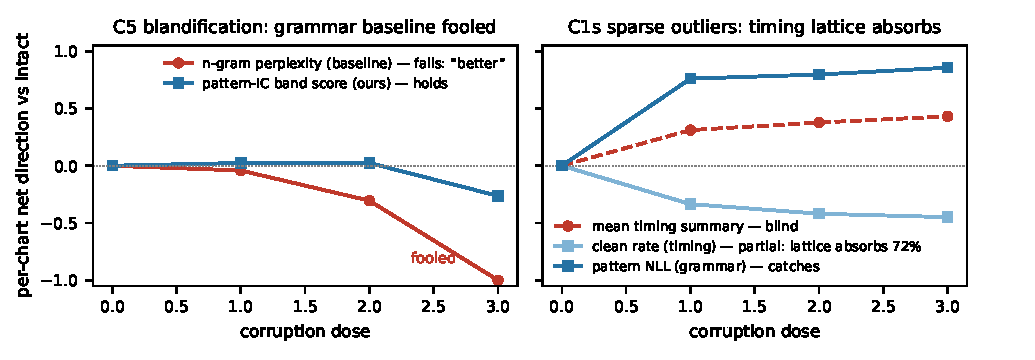
\includegraphics[width=0.92\textwidth]{figs/figA_complementarity.pdf}
\caption{Two cases in which one measurement misses a targeted change and
another responds. Bars show the fraction of charts moving up minus the
fraction moving down relative to the intact chart; light to dark marks
the three corruption strengths on the development panel (descriptive,
not independent-chart confidence statements). \textbf{Left:}
common-pattern rewriting lowers LM loss and raises the pattern-IC band
score, while the 4-gram repetition/uniqueness axis moves the other way
(its two algebraically equivalent output names are plotted once).
\textbf{Right:} sparse $\pm$60\,ms timing errors leave the mean timing
error near zero and are mostly re-paired by the nearest grid, while the
note-sequence LM responds to the changed intervals.}
\label{fig:complementarity}
\end{figure*}

Two borrowed metrics move in the nominally favorable direction under a
targeted corruption (\figref{fig:complementarity}, left).
\emph{Perplexity favors common patterns}: human development charts
average 9.44, while rewriting them toward the LM's most common patterns
lowers perplexity by 37\% (9.44 $\to$ 5.98). Dance
Dance Convolution reports perplexity as model fit on held-out human
charts~\cite{donahue2017ddc}; transplanted to generated output as a
reference-free quality reading, a lower-is-better interpretation favors
the rewritten chart. This is a chart-level example of the
likelihood/quality dissociation~\cite{theis2016note}. The reversal
remains when one LM creates the rewrite and another scores it
(9.44 $\to$ 6.04, $-$36\%). The pattern-IC band score moves toward its
human band and increases across the three doses. In the held-out
secondary analysis, its maximum-dose change is $+0.021$ with a nominal
95\% interval $[-0.034,0.077]$, while raw trigram NLL falls from 2.087
to 1.715 ($-0.373$, $[-0.399,-0.346]$). Typicality therefore does not
repair this case by itself. The effective 4-gram axis
(\secref{sec:dependency}) falls from 0.99 to 0.87 in development.

\emph{Self-similarity favors collapse}: replacing charts with their own dominant 4-gram loop
raises self-similarity structureness~\cite{wu2020jazz} by 62\% (0.0848
$\to$ 0.1370) and set-level Self-BLEU~\cite{zhu2018texygen} from 0.845
to 0.898. Copy-paste output is more self-similar by construction, while
the 4-gram repetition/uniqueness score falls from 0.99 to 0.83.

Two observational results complete the case. \emph{Direction
instability}: against the two publicly available taiko generators of
\secref{sec:systemresults}, whose outputs lie on the high-entropy side of the human corpus,
perplexity separates human from generated charts in the expected
direction (AUC 0.80), yet C5 shows that the
same reading inverts on the low-entropy side. A signed quality metric whose sign
depends on which side of the human distribution the system sits cannot
support a stable ranking; the same-difficulty band score treats both sides
symmetrically as deviations from typicality. C5 shows why that score
must be read together with the 4-gram repetition/uniqueness
axis. \emph{Length confounds}: on the same pool, type--token
ratio correlates with note count at $|\rho|=0.85$ and distinct-2 at
$0.56$, against at most $0.28$ for the band scores.

These cases establish complementarity without supplying aggregation
weights. We therefore keep the outputs separate instead of hiding their
trade-offs in one total. The complete metric--corruption response matrix appears in
Appendix~\figref{fig:responsemap}.

\subsection{Development evidence for the proposed components}
\label{sec:newmetricresults}

The five additional components in \tabref{tab:suite} have descriptive
development evidence. Their pooled Spearman responses across intact
charts and three doses support distinct operational roles. Reciprocity
falls under loop collapse and bar shuffling ($\rho=-.612$ and $-.506$)
while remaining nearly unchanged under timing jitter and global
translation ($-.086$ and $-.003$). The stagnation--alienation proxy
responds strongly to loop collapse ($\rho=-.924$ after orienting larger
as better) and changes little under timing jitter or global translation
($-.007$ and $+.010$). These results support sensitivity to the targeted
structural changes.

The two audio-response measures capture different scales. Run-head
onset support decreases under a global shift ($\rho=-.559$), whereas
bar-level density--energy response is stable under uniform density
scaling ($\rho=+.005$) and falls under bar shuffling ($\rho=-.386$).
Its weak burst-insertion response ($\rho=-.092$) confines the reading to
bar-scale covariation. The same-course human-chart distance describes a joint
feature distribution: it flags combinations unlike the training cloud
without classifying unusual charts as creative or poor. Its
course-conditioned score has maximum-dose net directions from $-.32$ to
$-.88$ under C3--C8 and a median change of zero under global
translation.

\subsection{System profiles}
\label{sec:systemresults}

The descriptive system profiles in \figref{fig:tiers} and
\figref{fig:profiles} separate two effects that a single number would
merge: similar headline timing fractions can arise from different
timing behavior, and the requested course can change the reading of
chart-side measurements.

\begin{figure*}[t]
\centering
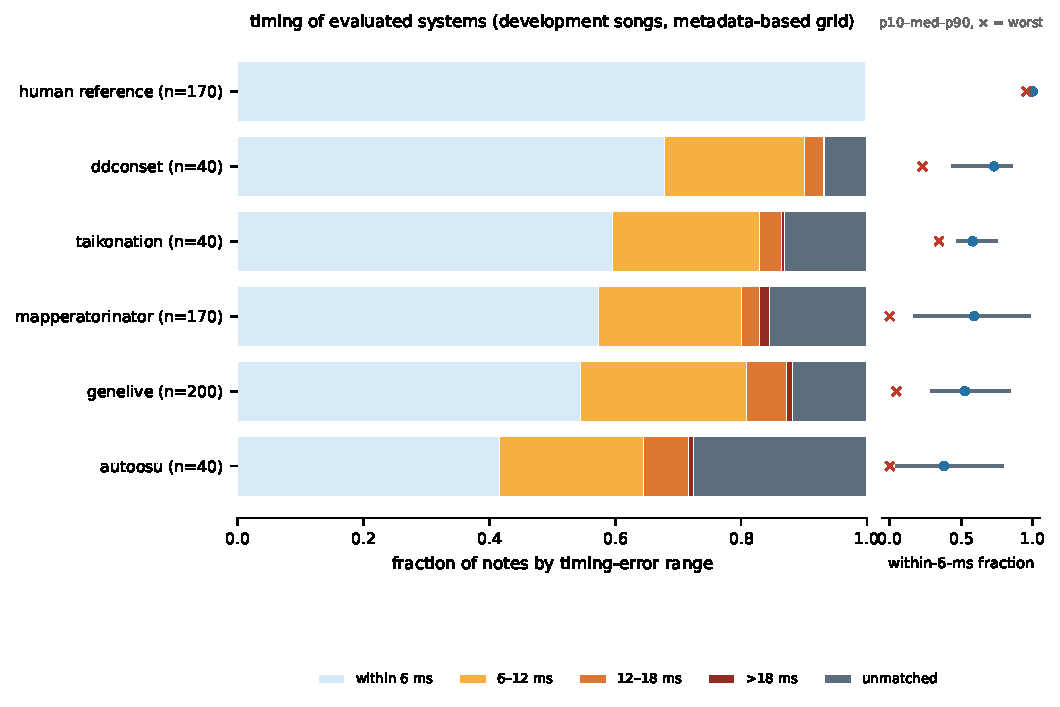
\includegraphics[width=0.92\textwidth]{figs/figB_timing_tiers.pdf}
\caption{Timing of the evaluated systems on the 40 development songs using
the authored grid. Each bar is the mean fraction of notes within 6\,ms
and in the 6--12, 12--18, and above-18\,ms ranges, or unmatched; $n$ is
the number of charts. In the right strip, the horizontal line spans the
10th--90th percentiles, the dot marks the median, and a downward triangle marks the
minimum within-6\,ms fraction. Similar mean clean fractions can coexist
with different timing tails.}
\label{fig:tiers}
\end{figure*}

\begin{figure*}[t]
\centering
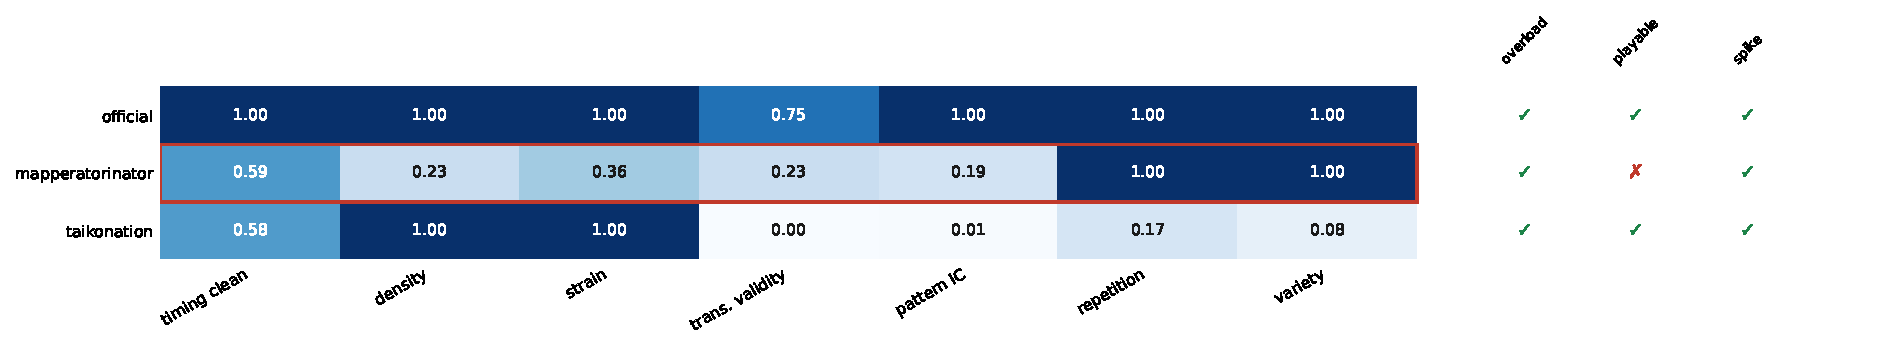
\includegraphics[width=0.92\textwidth]{figs/figD_profile_matrix.pdf}
\caption{Separate development results for the human reference and the two
generators that use Taiko note types. The first column is the median
fraction of notes within 6\,ms of the grid; the other cells are
calibrated scores in $[0,1]$. For note rate, short intervals, local
patterns, and the 4-gram repetition/uniqueness score, 1 means the median
lies within the human band; familiar transitions is one-sided (larger
better), and even the human reference reads 0.75 because an LM still
meets unseen trigrams. Symbols on the right show the overload, spike, and
playability checks at a median threshold of 0.5. Other note formats
appear only in the timing comparison (\figref{fig:tiers}). The separate
columns expose different departures; they are not combined into a total.}
\label{fig:profiles}
\end{figure*}

\textbf{Similar timing fractions can have different causes.} In
\figref{fig:tiers}, the near-unity human row is a consistency check on
using the authored bar metadata as the reference, not a model result.
The two
Taiko systems place nearly the same median fraction of notes within
6\,ms (0.59 and 0.58). Their remaining timing behavior differs.
Mapperatorinator places 10\% of adjacent intervals outside the relative
tolerance, compared with 41\% for TaikoNation. The grid-phase offset
search finds median offsets of 26 and 55\,ms, while nearest-grid matching
reports less than 1\,ms mean error beyond the 6\,ms tolerance for both.
TaikoNation also shows almost no
relation between chart activity and audio energy (correlation
$-0.003$), and its notes fall on average-energy frames. The DDC onset
system gives a 2.5\,ms offset on the same audio, serving as a control
against a shared decoding shift. AutoOsu, which shares
Mapperatorinator's osu! conversion path, reads a 19\,ms median offset;
the differing values rule out a shared conversion constant as the sole
explanation (\secref{sec:systems}).

\textbf{The requested course changes the reading.} Mapperatorinator's
generated-to-human note-rate ratio falls from 2.15--2.35 on Easy and
Normal to 1.31 on Oni and 1.07 on Ura
(Appendix~\figref{fig:difficulty}). Its note-rate, short-interval, and
local-pattern scores are below 0.5 on Easy through Hard and near 1 on
Oni and Ura. Timing does not follow the same trend: median fractions
within 6\,ms are 0.56, 0.60, 0.59, 0.57, and 0.62. The supported claim
is therefore a difficulty mismatch, not a general improvement
at high difficulty. TaikoNation exposes only one setting; at that
setting, note rate and short-interval load fit the human range, while
55\% of its trigrams are unseen in the course-conditioned training LM
and its repeated-4-gram rate is 0.004.

\section{Discussion}\label{sec:discussion}

ChartGenEval provides automatic six-dimensional feedback for chart
generators. The held-out tests show that seven effective output axes
respond to their targeted corruptions, while the development analyses
expose blind spots in common proxies. The profile can compare model
versions and show which dimension changed. Directional outputs can act
as rewards or penalties, playability checks as constraints, and
descriptive outputs as monitoring signals. A reinforcement-learning
setup can choose and weight these signals for its task.

\textbf{Atypicality requires context.} Controlled corruptions show that
targeted changes often move scores outside the same-course human band,
but the converse does not follow: an unusual chart may represent a
creative choice. Timing and feasibility checks help interpret that
departure. When signals disagree, the profile keeps the trade-off
visible.
The distance scale puts large departures in context: the development
human maximum is 4.8 half-range widths on the sequence axis, while the
Mapperatorinator and TaikoNation medians are 2.1 and 12.

\textbf{Transfer follows measurement roles.} Timing and music-response
measurements read only note times, which allowed direct application to
three note formats. Sequence, form, and distance measurements require a
tokenizer for the target game and human charts for calibration. Lane,
position, or direction tokens can replace Taiko note types, and the same
controlled-corruption design can test which responses transfer.
Position-based games additionally require movement-cost, hand-allocation,
and rotation checks.

\section{Limitations}\label{sec:limitations}

\textbf{Evidence scope.} Controlled corruptions show that measurements
respond to known changes; they do not directly measure player
experience. The nine corruptions omit
wrong-song pairing, deletion of musically important notes, and deliberate
off-grid placement. Individual charts may also move toward a human band
after a corruption. The five additional components have only
development-panel evidence. Finally, the two
prespecified C5 output names are algebraically equivalent; future work
should test an independent structure measurement.

\textbf{Corpus and system scope.} One game corpus defines the human
ranges. Its difficulty and tempo coverage is summarized in
Appendix~\figref{fig:coverage}. Other note formats receive only timing
and music-response measurements, and each public system runs in one
public configuration at one seed. Possible overlap between
development songs and system training corpora remains uncontrolled. The
shared-path comparison argues against one conversion constant as the
sole source of the observed offsets, but format-specific conversion
effects remain possible. The system results are therefore comparative
descriptions.

\textbf{Measurement and inference.} Timing clean rate penalizes added
off-grid notes but has no reference recall term, so deletion can improve
it; the measurement also requires an external grid. Held-out timing
results use the authored grid, while the audio-estimated alternative has
development evidence only. Sequence tokens include note intervals, so
timing and sequence responses can overlap
(Appendix~\figref{fig:responsemap}). Courses are averaged within song,
leaving songs as the inferential unit. Deterministic corruption
replicates are averaged within chart and do not create additional
samples.

\FloatBarrier

\section{Conclusion}\label{sec:conclusion}

We introduced ChartGenEval, a six-dimensional metric suite that uses the
matched official chart as an authored timing map while excluding its
note placements as targets. Timing is reported alongside five
higher-level dimensions; raw descriptions, two-sided typicality, and
one-sided feasibility checks retain separate roles, with no overall
score.

Nine nonredundant corruption--measurement pairs met the held-out
sensitivity and invariance criteria on 80 song groups. The same study
shows that chart-only measurements miss a global shift, while
perplexity and self-similarity can move favorably under targeted
corruptions.

The resulting profile provides automatic feedback for comparing and
iterating chart generators. Directional outputs can guide reward-based
optimization, feasibility checks can act as constraints, and
descriptive outputs can track model behavior. This role-based design
can support reinforcement learning while keeping each dimension
separate.

\section*{Ethics Statement}
The study uses community-transcribed charts and associated audio
gathered from online sources as described in \secref{sec:data}; these
potentially copyrighted materials are not redistributed. The released
materials exclude source charts, audio, personal data, and chart
generators. More capable evaluation can lower the cost of automated
content production; platform policy and moderation therefore remain
necessary for high-volume deployment.

\section*{AI Usage Statement}
AI assistants were used for experiment orchestration, drafting, and
editing under author direction; the author checked all reported values.

\appendix

\section{Corpus Coverage and Held-Out Evaluation Protocol}\label{app:protocol}

\subsection{Corpus coverage}

The calibration corpus is summarized by course, star level, and tempo.
\figref{fig:coverage} shows its difficulty and tempo coverage.

\begin{figure*}[t]
\centering
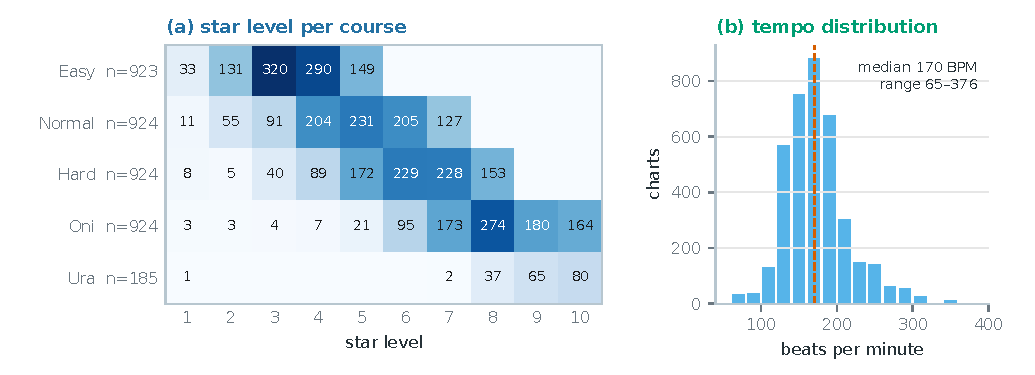
\includegraphics[width=0.98\textwidth]{figs/figCC_corpus_coverage.pdf}
\caption{Course difficulty and tempo coverage of the human reference corpus
that defines the calibration bands. \textbf{(a)} Star-level counts per course
across the 3{,}880 training charts: each course spans a broad, shifting
difficulty range. \textbf{(b)} Tempo histogram (median 170\,BPM, range
65--376).}
\label{fig:coverage}
\end{figure*}

\subsection{Panel construction and integrity}

Source rows are canonicalized by \texttt{group\_id} and audio SHA-256;
inconsistent aliases are rejected before panel indexing. The test split
contains 120 canonical song groups in stored order. Groups 0--39 form
the development panel, and groups 40--119 form the held-out panel.
Before inspecting held-out results, we fixed the dataset revision,
corruptions and doses, target measurements, controls, thresholds,
calibration, and analysis plan.

\subsection{Replicates, completeness, and inferential units}

Every nonzero corruption cell and control condition uses five fixed base
seeds. Replicates are averaged within chart and dose. A course is
complete only when its intact value, every target
dose and replicate, specified sham, and required controls are available. A
song enters a test with at least one complete course, and complete
courses are averaged within song. Songs, rather than charts, courses, or
replicates, are the inferential units for both response statistics.
Deterministic no-op and missing cells do not enter the analysis.

\subsection{Control checks and numerical invariance}

Identity re-evaluation applies to every retained measurement. A joint
+1-second shift of notes, authored grid, and duration tests invariance to
the time origin. A Don--Ka color bijection applies to timing and
density, where color is irrelevant; it is not a grammar or form control.
The 60\,ms C2 translation is the sham for chart-only density, grammar,
and structure measurements. A required control failure prevents support
for the affected target response. Each measurement uses a specified
equivalence tolerance and timestamp-rounding rule.
Chart-only interval arithmetic uses integer microseconds, three orders
of magnitude finer than the smallest reported tolerance.

\subsection{Intervals and decision rule}

After orienting outputs so that larger is better, the first statistic is
the within-chart Spearman correlation between the four severities
(intact plus three doses) and the measurement; an all-constant response
has zero sensitivity. The second statistic is the oriented
maximum-dose value minus the specified sham. Point estimates average
song-level values. We use 10{,}000 song-cluster bootstrap draws:
secondary analyses report nominal 95\% intervals, and the ten primary
rows use Bonferroni-adjusted 99.5\% intervals.
A response is supported when at least 72 of 80 songs are evaluable, all
controls pass, and both adjusted upper bounds are below zero. A
nonnegative adjusted lower bound contradicts the response; other cases
are inconclusive. The two C5 output rows were required to meet the rule
together, although their algebraic equivalence leaves one effective
axis. The C5 LM uses the full stored-order training split, trigram order
3, and add-$\alpha=0.05$.

\subsection{Sample counts and exclusions}

The held-out execution produced 50{,}283 observation records from 333
charts. C1s retained 332 complete courses and C8 retained 330; every
other effective pair retained 333. All 32 controls passed with maximum
observed absolute difference zero. Nineteen deterministic no-op cells
were excluded.

\FloatBarrier

\section{Controlled-Corruption Specifications}\label{app:corruptions}

\figref{fig:corruptionatlas} visualizes the operational change made by
each corruption and its prespecified target measurement.

\begin{figure*}[t]
\centering
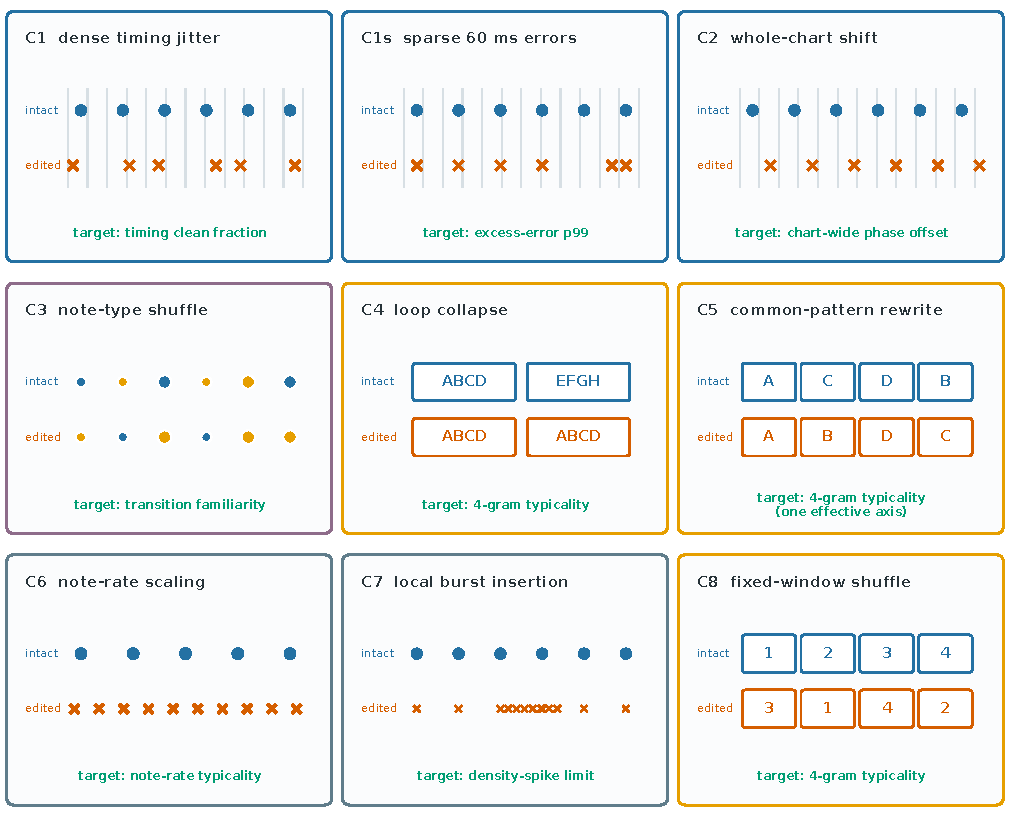
\includegraphics[width=0.98\textwidth]{figs/figP_corruption_atlas.pdf}
\caption{Controlled-corruption atlas. Blue marks the intact chart and
orange marks edited events. Each panel shows the property changed by one
corruption and names the target measurement. C1--C2 target timing, C3
targets transition familiarity, C4--C5 and C8 target repetition or
form, and C6--C7 target difficulty fit and local load. These edits
isolate operational changes; they do not exhaust chart quality.}
\label{fig:corruptionatlas}
\end{figure*}

The 170-chart development matrix uses one realization per nonzero cell,
producing 4{,}760 variants including the originals. C1s moves
$\max(1,\operatorname{round}(np))$ of a chart's $n$ notes by
$\pm60$\,ms. C3--C5 preserve note times, while C4 and C6 preserve or
control density. Raw features and their derived scores are evaluated on
the same variants; equivalent quantities are counted once. For C5, one
LM chooses common-pattern rewrites and an independently fitted LM scores
them. The perplexity reversal remains (9.44 $\to$ 6.04, $-36\%$).

\FloatBarrier

\section{Metric Guide and Extended Results}\label{app:visuals}

\figref{fig:metricguide} connects each construct to its required inputs,
representative outputs, and strongest present evidence. The evidence
labels distinguish outputs with held-out corruption tests from components
supported by development analyses.

\begin{figure*}[t]
\centering
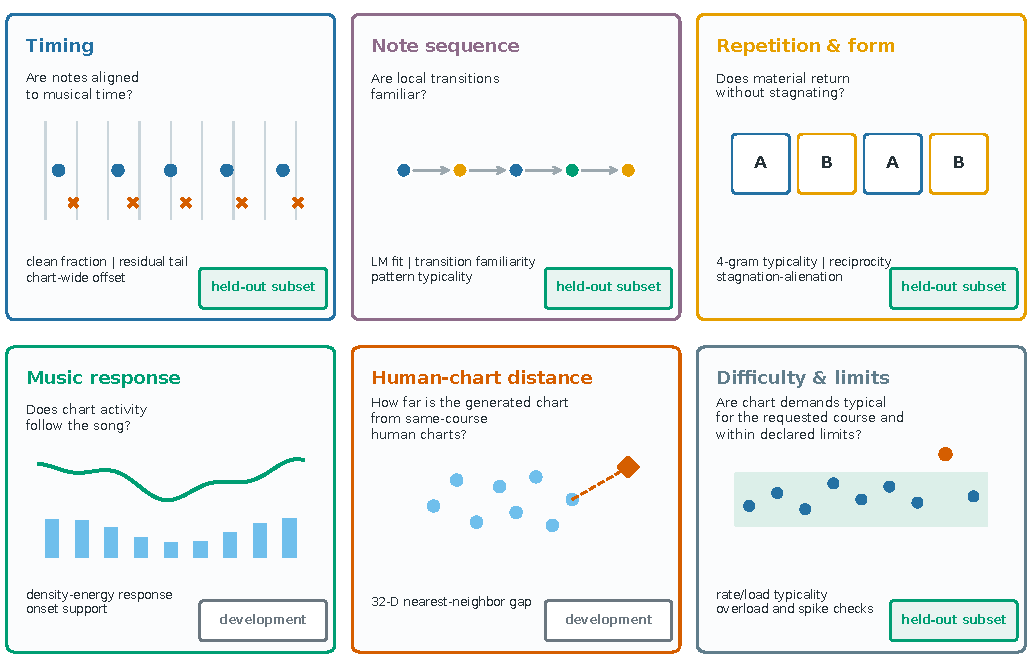
\includegraphics[width=0.98\textwidth]{figs/figM_metric_constructs.pdf}
\caption{Metric-to-construct guide. Each panel states an evaluation
question, illustrates the relevant signal, lists representative outputs,
and marks the strongest evidence. ``Held-out subset'' means that only
the named outputs in \tabref{tab:suite} have held-out corruption
evidence. Typicality describes departure from same-course human ranges.}
\label{fig:metricguide}
\end{figure*}

\figref{fig:responsemap} shows that targeted corruptions can affect
multiple score families, motivating interpretation as a profile rather
than as isolated interchangeable measurements.

\begin{figure*}[t]
\centering
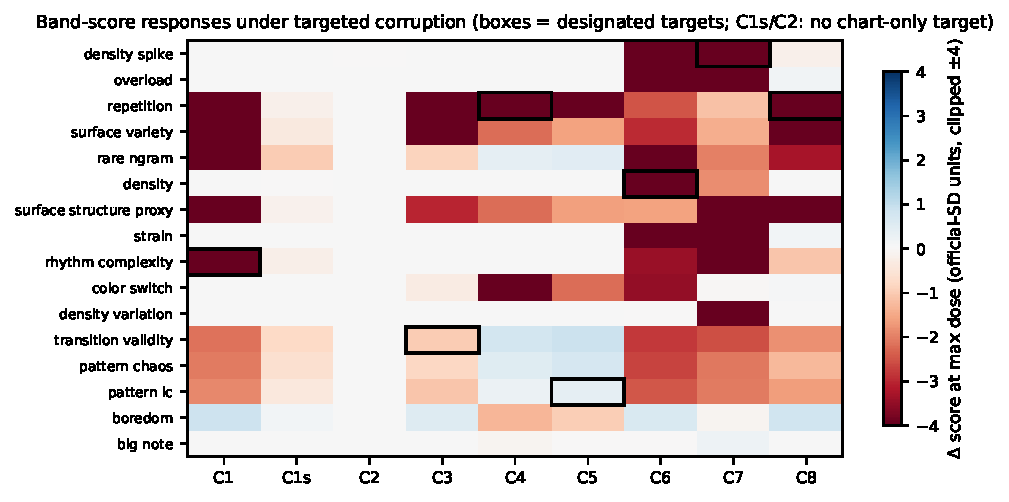
\includegraphics[width=0.94\textwidth]{figs/figC_coupling.pdf}
\caption{How 14 nonredundant calibrated chart-only scores respond to
each corruption at maximum strength on the development panel. Cells
cover band-typicality scores and one-sided checks. Red means the score
falls and blue that it rises; values are in standard deviations of the
human reference charts, clipped at $\pm4$. Black outlines mark the
target rows selected on the development panel; they do not mark
statistical significance. The matrix shows both target sensitivity and
cross-family coupling.}
\label{fig:responsemap}
\end{figure*}

\FloatBarrier

\begin{figure*}[t]
\centering
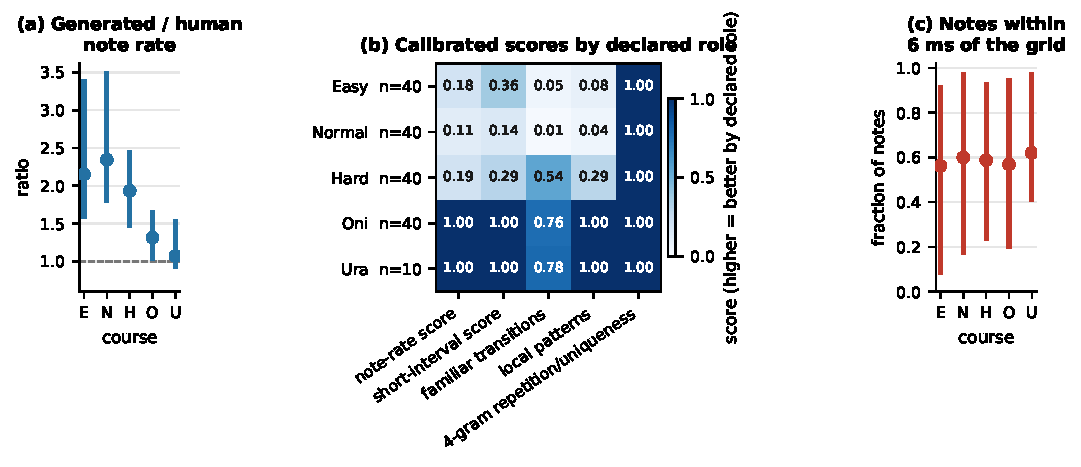
\includegraphics[width=0.96\textwidth]{figs/figE_difficulty.pdf}
\caption{Exploratory difficulty profile for Mapperatorinator on paired
development charts. Easy through Oni contain 40 song--course pairs; Ura
contains 10. Dots are medians and vertical lines span the 10th to 90th
percentiles. Generated density approaches the human reference as course
difficulty rises, while timing does not follow the same trend; this
supports a course mismatch rather than general improvement at high
difficulty.}
\label{fig:difficulty}
\end{figure*}

\FloatBarrier

\section{Released Materials}

Code, evaluation records, and plotting scripts are available at
\artifacturl.

\balance
\bibliographystyle{IEEEtran}
\bibliography{references}

\end{document}
